%%%%%%%%%%%%%%%%%%%%%%%%%%%%%%%%%%%%%%%%%
% Beamer Presentation
% LaTeX Template
% Version 1.0 (10/11/12)
%
% This template has been downloaded from:
% http://www.LaTeXTemplates.com
%
% License:
% CC BY-NC-SA 3.0 (http://creativecommons.org/licenses/by-nc-sa/3.0/)
%
%%%%%%%%%%%%%%%%%%%%%%%%%%%%%%%%%%%%%%%%%

%----------------------------------------------------------------------------------------
%	PACKAGES AND THEMES
%----------------------------------------------------------------------------------------

\documentclass{beamer}

\mode<presentation> {

% The Beamer class comes with a number of default slide themes
% which change the colors and layouts of slides. Below this is a list
% of all the themes, uncomment each in turn to see what they look like.

%\usetheme{default}
%\usetheme{AnnArbor}
%\usetheme{Antibes}
%\usetheme{Bergen}
%\usetheme{Berkeley}
%\usetheme{Berlin}
%\usetheme{Boadilla}
%\usetheme{CambridgeUS}
%\usetheme{Copenhagen}
%\usetheme{Darmstadt}
%\usetheme{Dresden}
%\usetheme{Frankfurt}
%\usetheme{Goettingen}
%\usetheme{Hannover}
%\usetheme{Ilmenau}
%\usetheme{JuanLesPins}
%\usetheme{Luebeck}
\usetheme{Madrid}
%\usetheme{Malmoe}
%\usetheme{Marburg}
%\usetheme{Montpellier}
%\usetheme{PaloAlto}
%\usetheme{Pittsburgh}
%\usetheme{Rochester}
%\usetheme{Singapore}
%\usetheme{Szeged}
%\usetheme{Warsaw}

% As well as themes, the Beamer class has a number of color themes
% for any slide theme. Uncomment each of these in turn to see how it
% changes the colors of your current slide theme.

%\usecolortheme{albatross}
%\usecolortheme{beaver}
%\usecolortheme{beetle}
%\usecolortheme{crane}
%\usecolortheme{dolphin}
%\usecolortheme{dove}
%\usecolortheme{fly}
%\usecolortheme{lily}
%\usecolortheme{orchid}
%\usecolortheme{rose}
%\usecolortheme{seagull}
%\usecolortheme{seahorse}
%\usecolortheme{whale}
%\usecolortheme{wolverine}

%\setbeamertemplate{footline} % To remove the footer line in all slides uncomment this line
%\setbeamertemplate{footline}[page number] % To replace the footer line in all slides with a simple slide count uncomment this line

%\setbeamertemplate{navigation symbols}{} % To remove the navigation symbols from the bottom of all slides uncomment this line
}
\usepackage{color}
\usepackage{xcolor}
\usepackage{listings}
\usepackage{graphicx} % Allows including images
\usepackage{booktabs} % Allows the use of \toprule, \midrule and \bottomrule in tables
\usepackage{polski}
\usepackage[utf8]{inputenc}
\usepackage{wrapfig}
\usepackage{subfigure}
\usepackage{amssymb}
\usepackage{amsmath}
\usepackage{hyperref}
\usepackage[belowskip=-15pt,aboveskip=0pt]{caption}
\usepackage{pgfplots}

\usepackage{placeins}

\usepackage{pgf}

\usepackage{tikz}

\usepackage{subfigure}
\usepackage{multicol}
\usepackage{color} %red, green, blue, yellow, cyan, magenta, black, white
\definecolor{mygreen}{RGB}{28,172,0} % color values Red, Green, Blue
\definecolor{mylilas}{RGB}{170,55,241}
\usepackage{listings}
\usepackage{amssymb}
\usepackage[T1]{fontenc}
\usepackage{libertine}
\newtheorem{twr}{Twierdzenie}
\makeatletter
% This command ignores the optional argument for itemize and enumerate lists
\newcommand{\inlineitem}[1][]{%
\ifnum\enit@type=\tw@
    {\descriptionlabel{#1}}
  \hspace{\labelsep}%
\else
  \ifnum\enit@type=\z@
       \refstepcounter{\@listctr}\fi
    \quad\@itemlabel\hspace{\labelsep}%
\fi}
\makeatother
\parindent=0pt
\lstdefinestyle{BashInputStyle}{
  language=bash,
  basicstyle=\small\sffamily,
  numbers=left,
  numberstyle=\tiny,
  numbersep=3pt,
  frame=tb,
  columns=fullflexible,
  backgroundcolor=\color{gray!20},
  linewidth=0.9\linewidth,
  xleftmargin=0.1\linewidth
}
\colorlet{punct}{red!60!black}
\definecolor{background}{HTML}{EEEEEE}
\definecolor{delim}{RGB}{20,105,176}
\colorlet{numb}{magenta!60!black}
\makeatletter
\newcommand{\lstuppercase}{\uppercase\expandafter{\expandafter\lst@token
                           \expandafter{\the\lst@token}}}
\newcommand{\lstlowercase}{\lowercase\expandafter{\expandafter\lst@token
                           \expandafter{\the\lst@token}}}
\makeatother

\lstdefinestyle{Oracle}{basicstyle=\ttfamily,
                        keywordstyle=\lstuppercase,
                        emphstyle=\itshape,
                        showstringspaces=false,
                        }
\lstdefinelanguage[Oracle]{SQL}[]{SQL}{
  morekeywords={ACCESS, MOD, NLS_DATE_FORMAT, NVL, REPLACE, SYSDATE,
                TO_CHAR, TO_NUMBER, TRUNC},
}
\definecolor{light-gray}{gray}{0.95}

\lstset{
  breaklines=true,                                     % line wrapping on
  language=SQL,
  frame=ltrb,
  framesep=2pt,
  basicstyle=\normalsize,
  keywordstyle=\ttfamily\color{green},
  identifierstyle=\ttfamily\color{blue}\bfseries,
  commentstyle=\color{Brown},
  stringstyle=\ttfamily,
  showstringspaces=ture,
  backgroundcolor=\color{light-gray},
  numbers=left
  }
  
  \lstset{language=Matlab,%
    %basicstyle=\color{red},
    breaklines=true,%
    morekeywords={matlab2tikz},
    keywordstyle=\color{blue},%
    morekeywords=[2]{1}, keywordstyle=[2]{\color{black}},
    identifierstyle=\color{black},%
    stringstyle=\color{mylilas},
    commentstyle=\color{mygreen},%
    showstringspaces=false,%without this there will be a symbol in the places where there is a space
    numbers=left,%
    numberstyle={\tiny \color{black}},% size of the numbers
    numbersep=3pt, % this defines how far the numbers are from the text
    emph=[1]{for,end,break},emphstyle=[1]\color{red}, %some words to emphasise
    %emph=[2]{word1,word2}, emphstyle=[2]{style},    
}


\lstdefinelanguage{json}{
    basicstyle=\normalfont\ttfamily,
    numbers=left,
    numberstyle=\tiny,
    stepnumber=1,
    numbersep=1pt,
    showstringspaces=false,
    breaklines=true,
    frame=lines,
    backgroundcolor=\color{background},
    literate=
     *{0}{{{\color{numb}0}}}{1}
      {1}{{{\color{numb}1}}}{1}
      {2}{{{\color{numb}2}}}{1}
      {3}{{{\color{numb}3}}}{1}
      {4}{{{\color{numb}4}}}{1}
      {5}{{{\color{numb}5}}}{1}
      {6}{{{\color{numb}6}}}{1}
      {7}{{{\color{numb}7}}}{1}
      {8}{{{\color{numb}8}}}{1}
      {9}{{{\color{numb}9}}}{1}
      {:}{{{\color{punct}{:}}}}{1}
      {,}{{{\color{punct}{,}}}}{1}
      {\{}{{{\color{delim}{\{}}}}{1}
      {\}}{{{\color{delim}{\}}}}}{1}
      {[}{{{\color{delim}{[}}}}{1}
      {]}{{{\color{delim}{]}}}}{1},
}
\definecolor{gray}{rgb}{0.4,0.4,0.4}
\definecolor{darkblue}{rgb}{0.0,0.0,0.6}
\definecolor{cyan}{rgb}{0.0,0.6,0.6}
\lstdefinelanguage{XML}
{
tabsize=3,
  morestring=[b]",
  morestring=[s]{>}{<},
  morecomment=[s]{<?}{?>},
  stringstyle=\color{black},
  identifierstyle=\color{darkblue},
  keywordstyle=\color{cyan},
   backgroundcolor=\color{background},
  morekeywords={xmlns,version,type}% list your attributes here
}
%----------------------------------------------------------------------------------------
%	TITLE PAGE
%----------------------------------------------------------------------------------------
\institute[AGH] % Your institution as it will appear on the bottom of every slide, may be shorthand to save space
{
 % Your institution for the title page
\medskip

\includegraphics[scale=0.2]{agh}\\
\textsc{\scriptsize Akademia Górniczo-Hutnicza im. Stanisława Staszica w Krakowie}\\[0.2 cm] % Name of your university/college
{\Large Wydział Fizyki i Informatyki Stosowanej}\\
} 
\title[JSON in PostgreSQL database]{JSON w bazie danych PostgreSQL} % The short title appears at the bottom of every slide, the full title is only on the title page

\author[Maciej Kubicki]{Maciej Kubicki}


% Your email address
%\titlegraphic{
\includegraphics[scale=0.2]{agh}}
 % Date, can be changed to a custom date



\begin{document}

\begin{frame}
\titlepage % Print the title page as the first slide
\end{frame}

\begin{frame}
\frametitle{Spis treści} % Table of contents slide, comment this block out to remove it
\tableofcontents % Throughout your presentation, if you choose to use \section{} and \subsection{} commands, these will automatically be printed on this slide as an overview of your presentation
\end{frame}

\section{Cel pracy}
\begin{frame}
\frametitle{Cel pracy oraz użyte narzędzia}
 Celem pracy jest przedstawienie możliwości formatu JSON zaimplementowanego w relacyjnej bazie danych jaką jest PostgreSQL oraz porównanie tychże narzędzi z innymi rozwiązaniami NoSQL-owymi. 
 \vspace{1cm}\newline
 W pracy inżynierskiej używałem PostgreSQL 9.6.1, MongoDB 3.2.1, Couchbase Server Enterprise 4.5.1 oraz Python 2.7 wraz z odpowiednimi bibliotekami.

\end{frame}

\section{Dane testowe}
\subsection{Pierwszy zestaw danych}
\begin{frame}[fragile]
\frametitle{Pierwszy zestaw testowy}
{\small Pierwszy zestaw został wygenerowany na podstawie AdvenutreWorks2008 z Microsoft SQL Server. Oto kod, który wygenerował zbiór 18798 dokumentów JSON. }
\begin{lstlisting}[language=Python,basicstyle=\scriptsize]
from DatabasePrepartion import *
import pyodbc 
cnxn = pyodbc.connect('DRIVER={SQL Server};SERVER=localhost\SQLEXPRESS;DATABASE=AdventureWorks2008;')
cursor = cnxn.cursor()
cursor.execute("SELECT e.EmailAddress, pp.FirstName, ISNULL(pp.MiddleName,'') AS MiddleName, pp.LastName, p.BusinessEntityID,[AddressLine1],ISNULL([AddressLine2],'') AS AddressLine2,[City],[PostalCode] FROM [AdventureWorks2008].[Person].[Address] a,[AdventureWorks2008].[Person].[EmailAddress] e, [AdventureWorks2008].[Person].[BusinessEntityAddress] p, [AdventureWorks2008].[Person].[Person] pp WHERE p.AddressID = a.AddressID and pp.BusinessEntityID=p.BusinessEntityID and e.BusinessEntityID=pp.BusinessEntityID;")
rows = cursor.fetchall()
with open('person.json','w') as pl:
	for row in rows:
		if is_json(to_json(row) ):
			pl.write(to_json(row,False)+'\n')
\end{lstlisting}

\end{frame}

\begin{frame}[fragile]
\frametitle{Pierwszy zestaw testowy}
{\small Funkcja to\_json na podstawie wyniku wiersza generuje dokument JSON. Struktura wygenerowanych dokumentów nie jest jednakowa. Mianowicie nie każdy człowiek (odpowiadający mu dokument) posiada klucz MiddleName oraz address\_line2. Dodatkowo liczba adresów e-mail przypisanych do osoby może wynosić 0,1,2. }
\begin{lstlisting}[language=JSON,basicstyle=\scriptsize]
{
	"person": {
		"personID": 12,
		"FirstName": "Thierry",
		"MiddleName": "B",
		"LastName": "DHers"
	},
	"addres": {
		"city": "Bothell",
		"addres_line1": "1970 Napa Ct.",
		"postal_code": "98011"
	},
	"email": ["thierry0@adventure-works.com", "DHers12@mail.com"]
}
\end{lstlisting}
\captionof{lstlisting}{Wygenerowany dokument JSON}\vspace{0.5cm}

\end{frame}
\begin{frame}[fragile]
\frametitle{Pierwszy zestaw testowy - PostgreSQL}
\begin{lstlisting}[language=SQL]
CREATE TABLE PersonJSONB (
  "ObjectID" SERIAL   NOT NULL ,
  data JSONB NOT NULL,
PRIMARY KEY("ObjectID"));
CREATE TABLE PersonJSON(
  "ObjectID" serial NOT NULL,
  data JSON NOT NULL,
PRIMARY KEY ("ObjectID"));
\end{lstlisting}
\captionof{lstlisting}{Tworzenie tabeli w PostgreSQL z typami jsonb i json}\vspace{0.5cm}

\end{frame}

\subsection{Drugi zestaw danych}
\begin{frame}[fragile]
\frametitle{Drugi zestaw testowy - PostgreSQL}

\begin{lstlisting}[language=SQL]
CREATE TYPE Gender AS ENUM('M','F');
CREATE TABLE Users (
  idUsers SERIAL   NOT NULL ,
  username VARCHAR(20)   NOT NULL ,
  password VARCHAR(255)   NOT NULL ,
  mail VARCHAR(255)   NOT NULL ,
  Name VARCHAR   NOT NULL ,
  Surname VARCHAR   NOT NULL ,
  town VARCHAR(20)   NOT NULL ,
  gender Gender   NOT NULL ,
  country VARCHAR(255) NOT NULL,
PRIMARY KEY(idUsers));
\end{lstlisting}
\captionof{lstlisting}{Tworzenie tabeli z drugim zestawem danych}\vspace{0.5cm}

\end{frame}
\section{JSON w PostgreSQL}
\begin{frame}
\frametitle{JSON w PostgreSQL}
Funkcjonalność wspierająca JSON w PostgreSQL-u:
\begin{itemize}
\item Typy danych obsługujące format JSON: json i jsonb,
\item Operatory działające na powyższych typach,
\item Funkcje przetwarzające dokumenty JSON,
\item Funkcje tworzące dokumenty JSON,
\item Indeksy na kluczach dokumentów JSON.
\end{itemize}
\end{frame}
\subsection{Operatory}
\begin{frame}[fragile]
\frametitle{Operatory}
Jakie? Do czego służą?
\begin{lstlisting}[language=SQL,basicstyle=\footnotesize]
SELECT "ObjectID", data->'person'->>'LastName' AS Surname FROM personjsonb WHERE data->'person'->>'LastName' LIKE 'T%' LIMIT 5;
\end{lstlisting}
\captionof{lstlisting}{Przykład użycia operatorów}\vspace{0.5cm}
\begin{figure}[h]
\begin{center}
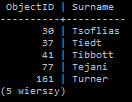
\includegraphics[scale=1.1]{sc/1}
\end{center}
\caption{Wynik zapytania z przykładu}
\end{figure}
\end{frame}
\subsection{Funkcje przetwarzające}
\begin{frame}[fragile]
\frametitle{Funkcje przetwarzające}
\begin{lstlisting}[language=SQL,basicstyle=\tiny]
SELECT jsonb_pretty(data) FROM public.personjsonb WHERE "ObjectID"=1922;
UPDATE public.personjsonb SET data = (SELECT jsonb_set(data,'{email,1}','"newmail@hotmail.com"',false) FROM public.personjsonb WHERE "ObjectID"=1922) WHERE "ObjectID"=1922;
SELECT jsonb_pretty(data) FROM public.personjsonb WHERE "ObjectID"=1922;
\end{lstlisting}
\captionof{lstlisting}{Przykład przetwarzania}\vspace{0.65cm}
\begin{minipage}{0.49\textwidth}
\makeatletter
\def\@captype{figure}
\makeatother
\begin{center}
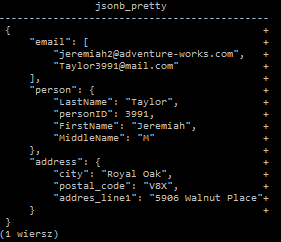
\includegraphics[scale=0.7]{sc/36}
\caption{Przed modyfikacją}
\end{center}

\end{minipage}
\begin{minipage}{0.4\textwidth}
\makeatletter
\def\@captype{figure}
\makeatother
\begin{center}
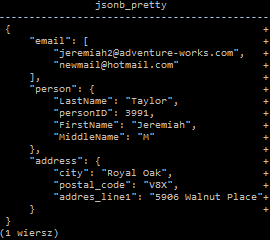
\includegraphics[scale=0.7]{sc/37}
\caption{Po modyfikacji}
\end{center}
\end{minipage}
\end{frame}
\subsection{Funkcje tworzące}
\begin{frame}[fragile]
\frametitle{Funkcje tworzące}
Jakie? Po co?
\begin{lstlisting}[language=SQL,basicstyle=\footnotesize]
SELECT row_to_json(row,true) FROM (SELECT idUsers,username, Name, Surname, mail FROM Users WHERE idUsers=4) row;
\end{lstlisting}
\captionof{lstlisting}{Przykład tworzenie dokumentu JSON}\vspace{0.5cm}
\begin{figure}[h]
\begin{center}

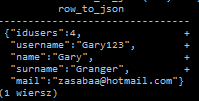
\includegraphics[scale=1]{sc/44}

\end{center}
\caption{Wynik z przykładu}
\end{figure}



\end{frame}
\subsection{Indeksy}
\begin{frame}[fragile]
\frametitle{Używanie indeksów w dokumentach JSON}
\begin{lstlisting}[language=SQL,basicstyle=\tiny]
SELECT "ObjectID", data->'person'->>'LastName'::text AS Surname FROM personjsonb WHERE data->'person'->>'LastName'::text LIKE 'T%';
CREATE INDEX surname on personjsonb (((data->'person'->>'LastName')::text));
SELECT "ObjectID", data->'person'->>'LastName'::text AS Surname FROM personjsonb WHERE data->'person'->>'LastName'::text LIKE 'T%';
\end{lstlisting}
\captionof{lstlisting}{Przykład użycia indeksów}
\begin{figure}[h]
\begin{center}
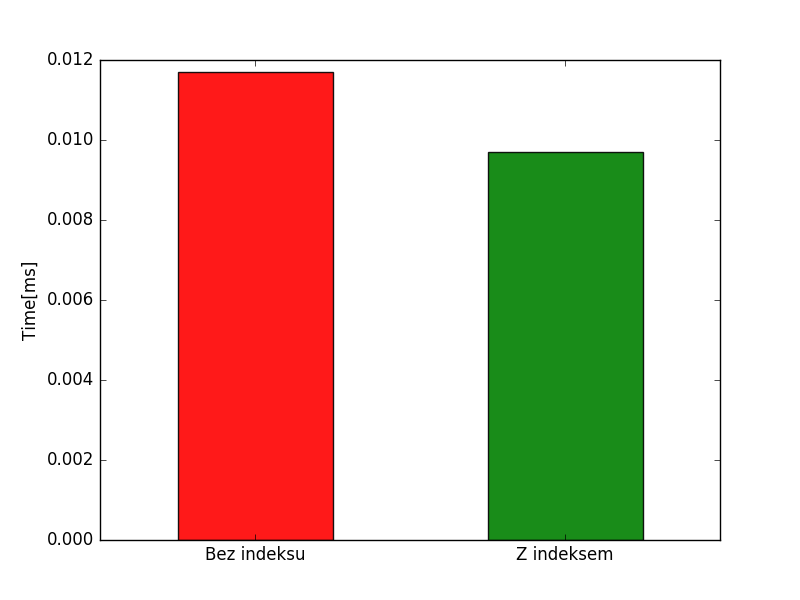
\includegraphics[scale=0.36]{ax/figindex}
\end{center}
\caption{Czas wykonania przykładowego zapytania z użyciem i bez użycia indeksu}
\end{figure}
\end{frame}
\section{Porównanie obsługi JSON w PostgreSQL z rozwiązaniami NoSQL}

\begin{frame}[fragile]
\subsection{Wprowadzanie danych}
\frametitle{Porównanie - wprowadzanie danych}
\begin{lstlisting}[language=SQL,basicstyle=\tiny]
\i 'person_insert_jsonb.sql'
\i 'person_insert_json.sql'
mongoimport --db test --collection person_col --drop < person.json
cbdocloader -n localhost:8091 -u Administrator -p password -b Person_Bucket Person_Bucket.zip
\end{lstlisting}
\begin{figure}[h]
\begin{center}
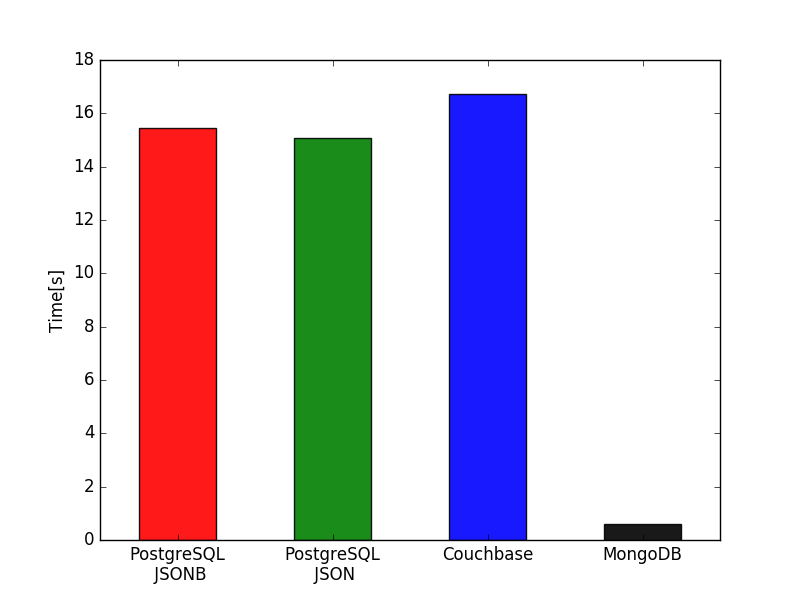
\includegraphics[scale=0.37]{ax/fig0}
\end{center}
\caption{Czas wprowadzania danych do poszczególnych baz}
\end{figure}

\end{frame}

\begin{frame}[fragile]
\subsection{Przeszukiwanie danych}
\frametitle{Porównanie - przeszukiwanie danych}
\begin{lstlisting}[language=SQL,basicstyle=\tiny]
SELECT max(cast(data->'person'->>'personID' AS int)) FROM personjsonb;
SELECT max(cast(data->'person'->>'personID' AS int)) FROM personjson;
SELECT max(person.personID) FROM `Person_Bucket`;
db.person_col.find({},{"person.personID":1}).sort({"person.personID": -1}).limit(1)
\end{lstlisting}
\begin{figure}[h]
\begin{center}
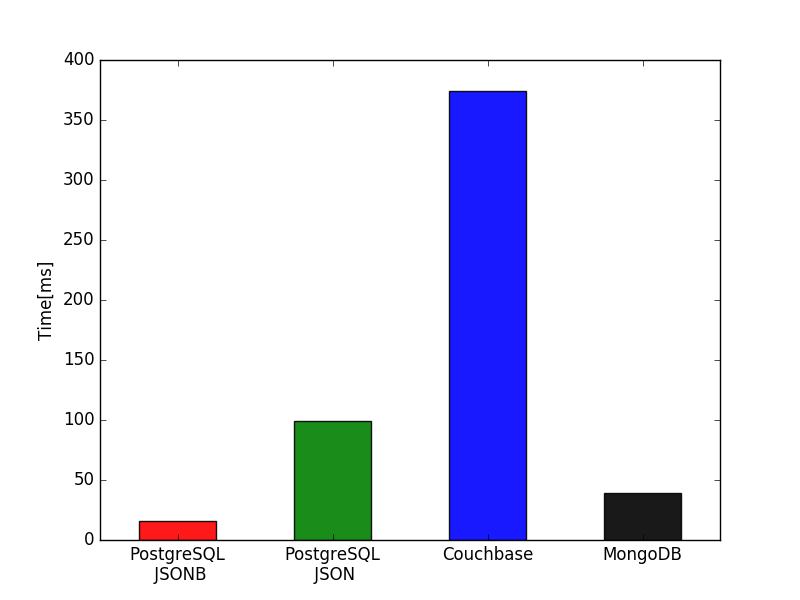
\includegraphics[scale=0.37]{ax/fig1}
\end{center}
\caption{Czas wyszukiwania w poszczególnych bazach}
\end{figure}

\end{frame}

\begin{frame}[fragile]
\subsection{Modyfikacja danych}
\frametitle{Porównanie - modyfikowanie danych}
W tym przykładzie modyfikacja polega na dodaniu tablicy "email", wraz z jedną wartością do dokumentów, w których nie ma takie tablicy.

\begin{figure}[h]
\begin{center}
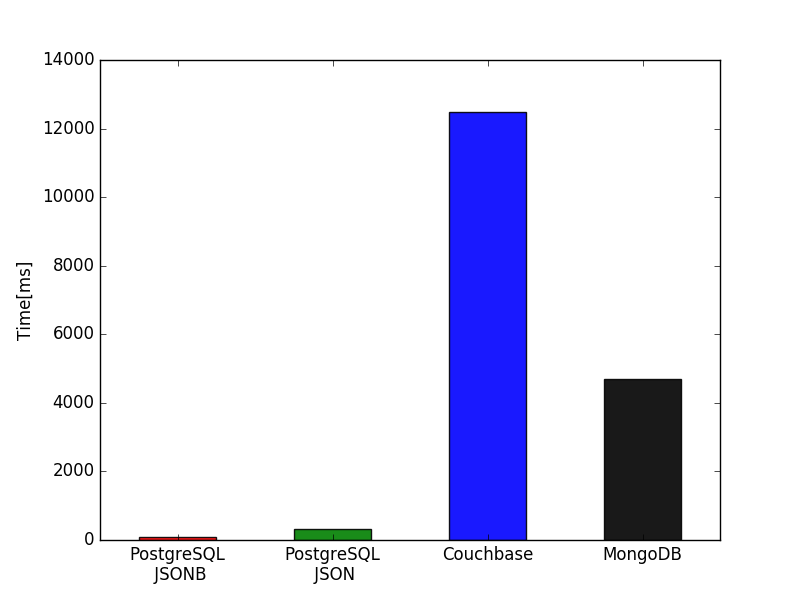
\includegraphics[scale=0.37]{ax/fig5}
\end{center}
\caption{Czas modyfikacji w poszczególnych bazach}
\end{figure}

\end{frame}

\begin{frame}[fragile]
\subsection{Rozmiar danych}
\frametitle{Porównanie - rozmiar danych}

\begin{figure}[h]
\begin{center}
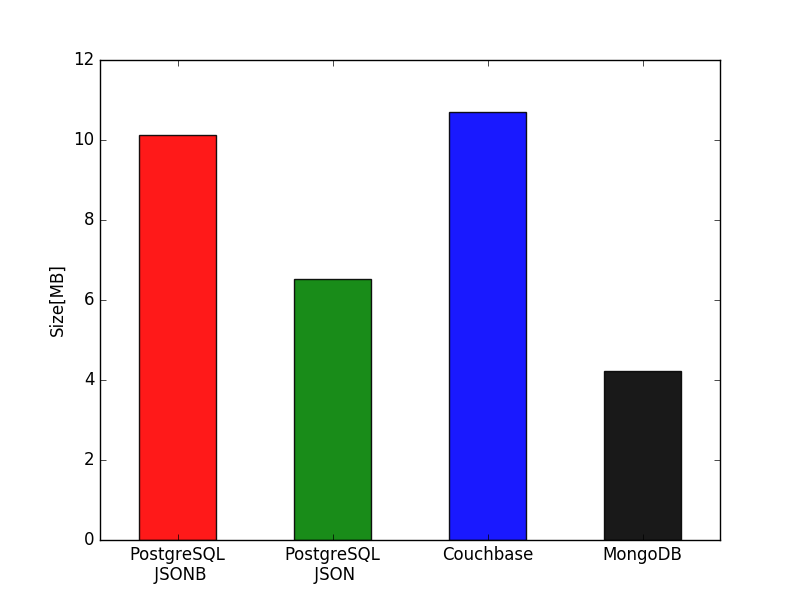
\includegraphics[scale=0.37]{ax/fig7}
\end{center}
\caption{Rozmiar danych w poszczególnych bazach}
\end{figure}

\end{frame}

\subsection{Wnioski}
\begin{frame}
\frametitle{Wnioski}
W przypadku wprowadzania danych zdecydowanym liderem okazała się baza MongoDB, która wyprzedza pozostałe rozwiązania. Potwierdziła się teza zgodnie, z którą json (PostgreSQL) jest szybszy we wprowadzaniu danych od jsonb (minimalnie), a wolniejszy w ich przetwarzaniu. Prawie we wszystkich testach najwolniej działał Couchbase, jednak prawie wszystkie testy zakładały użycie N1QL, a więc zmuszony byłem do korzystania z Couchbase Bucket (alternatywą jest Memcached Bucket, który nie wspiera N1QL). Typ jsonb z PostgreSQL i baza MongoDB działają ze zbliżoną prędkością jeśli chodzi o przeszukiwanie danych i ich grupowanie, a json jest trochę wolniejszy. W aspekcie aktualizacji i kasowania danych najwydajniej pracuje Postgres. Ostatnim przypadkiem testowym był pomiar rozmiaru zajętego na dysku. Najkorzystniej wypadła baza MongoDB.
\end{frame}
\end{document}
